% -----------------------------------------------
% Template for ISMIR Papers
% 2015 version, based on previous ISMIR templates
% -----------------------------------------------

\documentclass{article}
\usepackage{ismir,amsmath,cite}
\usepackage{url}
\usepackage{graphicx}
\usepackage{color}
\usepackage{cleveref}
\usepackage{authblk}
\usepackage{dsfont}

\graphicspath{{figs/}}

% Title.
% ------
\title{Four Timely Insights on Automatic Chord Estimation}

% Two addresses
% --------------
% \twoauthors
%  {Eric J. Humphrey} {MARL  \\ Department}
%  {Second author} {Company \\ Address}

% Three addresses
% --------------
% \threeauthors
%   {First author} {Affiliation1 \\ {\tt author1@ismir.net}}
%   {Second author} {\bf Retain these fake authors in\\\bf submission to preserve the formatting}
%   {Third author} {Affiliation3 \\ {\tt author3@ismir.net}}

\author[1,2]{Eric J. Humphrey}
\author[1]{Juan P. Bello}
\affil[1]{Music and Audio Research Laboratory, New York University}
\affil[2]{MuseAmi, Inc.}

\def\authorname{Eric J. Humphrey, Juan P. Bello}

\begin{document}
%
\maketitle
\sloppy
%

\let\oldthefootnote\thefootnote%
\renewcommand{\thefootnote}{\fnsymbol{footnote}}
\footnotetext[1]{Please direct correspondence to \url{eric@museami.com}}
\let\thefootnote\oldthefootnote%

\begin{abstract}

Automatic chord estimation (ACE) is a hallmark research topic in content-based music informatics, but like many other tasks, system performance appears to be converging to yet another glass ceiling.
Looking toward trends in other machine perception domains, one might conclude that complex, data-driven methods have the potential to significantly advance the state of the art.
Two recent efforts did exactly this for large-vocabulary ACE, but despite arguably achieving some of the highest results to date, both approaches plateau well short of having solved the problem.
Therefore, this work explores the behavior of these two high performing,  systems as a means of understanding obstacles and limitations in chord estimation, arriving at four critical observations:
one, music recordings that invalidate tacit assumptions about harmony and tonality result in erroneous and even misleading performance;
two, standard lexicons and comparison methods struggle to reflect the natural relationships between chords;
three, conventional approaches conflate the competing goals of recognition and transcription to some undefined degree;
and four, the perception of chords in real music can be highly subjective, making the very notion of ``ground truth'' annotations tenuous.
Synthesizing these observations, this paper offers possible remedies going forward, and concludes with some perspectives on the future of both ACE research and the field at large.

\end{abstract}


\section{Introduction}
\label{sec:introduction}

% Chord rec is standard in the community
Among the various subtopics in content-based music informatics, automatic chord estimation (ACE) has matured into a classic MIR challenge, receiving healthy attention from the research community for the better part of two decades.
%, people want / need
Complementing our natural sense of academic intrigue, the general music learning public places a high demand on chord-based representations of popular music, as evidenced by large online communities surrounding websites like e-chords\footnote{\url{http://www.e-chords.com}} or Ultimate Guitar\footnote{\url{http://www.ultimate-guitar.com}}.
% ...but this is difficult
Given the prerequisite skill necessary to manually identify chords from recorded audio, there is considerable motivation to develop automated systems capable of reliably performing this task.


The goal of ACE research is ---or, at least, has been--- to develop systems that produce ``good'' time-aligned sequence of chords from a given music signal.
Supplemented by efforts in data curation \cite{Burgoyne2011Expert}, syntax standardization \cite{Harte2005Symbolic}, and evaluation \cite{Pauwels2013Evaluating}, the bulk of chord estimation research has concentrated on building better systems, mostly converging to a common architecture \cite{Cho2014Relative}:
%, diagrammed in Figure \ref{fig:basic_ace}
first, harmonic features, referred to as pitch class profiles (PCP) or \emph{chroma}, are extracted from short-time observations of the audio signal \cite{Fujishima1999Realtime};
these features may then be processed by any number of means, referred to in the literature as \emph{pre-filtering};
next, \emph{pattern matching} is performed independently over observations to measure the similarity between the signal and a set of pre-defined chord classes, yielding a time-varying likelihood;
and finally, \emph{post-filtering} is applied to this chord class posterior, resulting in a sequence of chord labels over time.

However, despite continued efforts to develop better features \cite{Mueller2010Towards}, more powerful classifiers \cite{Humphrey2012Rethinking}, or advanced post-filtering methods \cite{Boulanger2013Audio}, performance appears to be tapering off, as evidenced by recent years' results at MIReX\footnote{\url{http://www.music-ir.org/mirex/wiki/MIREX\_HOME}}.
Thus, while other areas of machine perception, such as computer vision and speech recognition, are able to leverage modern advances in machine learning with remarkable success, two recent efforts in large vocabulary ACE were only able to realize modest improvements by comparison \cite{Cho2014Improved, Humphrey2015Exploration}.
Acknowledging this situation begs an obvious question:
why is automatic chord estimation different, and what might be done about it?
% --- ---  --- ---
Through an investigation of system behaviour and detailed error analysis, the remainder of this paper is an effort to shed some light on the problem.
% first, \Cref{sec:method} details the research methodology used here, covering the choice of automatic systems, objective evaluation, and the datasets considered;
% \Cref{sec:experiment} introduces a large-vocabulary chord estimation experiment and the corresponding high-level results;
% then, to develop a deeper understanding of how these systems behave and the kinds of errors that they make, \Cref{sec:analysis} identifies four critical insights, indicating that performance ceilings may be as much a function of traditional ACE methodology as the automatic systems being considered;
% finally, \Cref{sec:perspectives} offers perspectives to help frame future work.


\section{Research Methodology}
\label{sec:method}

\subsection{Automatic Systems}
\label{subsec:systems}

Given its long history, there are ample potential automatic chord estimation systems that could be considered in this inquiry.
Here, though, we choose to focus our investigation on two recent, data-driven, large vocabulary systems for which we are able to obtain software implementations, providing control over training and choice of chord vocabulary.
Additionally, these system architectures are quite different and should, as a result, yield different machine perspectives, a strategy that has proven useful in the analysis of beat tracking systems \cite{Zapata2012Assigning}.


\subsubsection{K-stream GMM-HMM with Multiband Chroma}
\label{subsubsec:kHMM}

The first system considered is a modern, high-performing GMM/HMM chord estimation system \cite{Cho2014Improved}, referred to here as ``kHMM.''
A multiband chroma representation is computed from beat-synchronous audio analysis, producing four parallel feature representations.
Each is modeled by a separate multivariate Gaussian Mixture Model (GMM), whereby all chroma vectors and chord labels are rotated to a \texttt{C} root.
During inference, four separate observation likelihoods over all chord classes are obtained by circularly rotating the feature vector the GMM, thereby making the model transposition invariant.
These four chord class posteriors are then decoded jointly using a k-stream HMM, resulting in a single beat-aligned chord sequence.


\subsubsection{Deep Convolutional Neural Network}
\label{subsubsec:DNN}

Acknowledging the recent widespread success of deep learning methods, a deep convolutional network is also considered \cite{Humphrey2015Exploration}, referred to as ``DNN.''
Time-frequency patches of local contrast normalized constant-Q spectra, on the order of one second, are transformed by a four-layer convolutional network.
Finding inspiration in the root-invariance strategy of GMM training, explicit weight-tying is achieved at the classifier across roots such that all qualities develop the same internal representations, allowing the model to generalize to chords unseen during training.
Following the lead of deep network research in automatic speech recognition, likelihood scaling is performed after training to control class bias resulting from the severe imbalance in the distribution of chords.
Finally, chord posteriors are decoded via the Viterbi algorithm \cite{Cho2010Exploring}.


\subsection{Evaluation}
\label{subsec:eval}

Expressed formally, the modern approach to scoring an ACE system is a weighted measure of chord-symbol recall, $R_{W}$, between a reference, $\mathcal{R}$, and estimated, $\mathcal{E}$, chord sequence as a continuous integral over time, summed over a discrete collection of $N$ annotation pairs:

\begin{equation}
\label{eq:recall_micro}
R_{W} = \frac{1}{S}\sum_{n=0}^{N-1}\int_{t=0}^{T_n}C(\mathcal{R}_n(t), \mathcal{E}_n(t))~dt
\end{equation}

\noindent Here, $C$ is a chord \emph{comparison} function, bounded on $[0, 1]$, $t$ is time, $n$ the index of the track in a collection, $T_n$ the duration of the $n^{th}$ track. This total is normalized by the \emph{support}, $S$, corresponding to the cumulative amount of time over which the comparison rule is defined for $\mathcal{R}$, given by the indicator function in a similar integral:

\begin{equation}
S = \sum_{n=0}^{N-1}\int_{t=0}^{T_n}\mathds{1}_{\mathcal{R}_n(t)}~dt
\end{equation}

Defining the normalization term $S$ separately is useful when comparing chord names, as it relaxes the assumption that the comparison function is defined everywhere.
Furthermore, setting the comparison function as a free variable allows for flexible evaluation of a system's outputs, and thus the focus on vocabulary can largely focus on the choice of comparison function, $C$.
The work presented here leverages \texttt{mir\_eval}, an open source evaluation toolbox providing a set of seven chord comparison functions, characterizing different relationships between chords \cite{Raffel2014Eval}.


\subsection{Reference Annotations}
\label{subsec:data}

% TODO: Clean this up.
% Subjective evaluation is costly, and thus researchers have long sought to characterize ACE performance via objective means.
% Identify data for training and evaluation.
% Two kinds of data; ground truth for training and test, curated specifically for ACE research.


\subsubsection{Ground Truth Data}
\label{subsubsec:ground_truth}

The first major effort to curate reference chord annotations, now part of the larger Isophonics\footnote{\url{http://isophonics.net/content/reference-annotations}} dataset, covers the entire 180-song discography of \emph{The Beatles}, as well as 20 songs from \emph{Queen}, 14 from Carole King, and 18 from \emph{Zweieck};
due to content access, only the 200 songs from \emph{The Beatles} and \emph{Queen} are used here.
Two other large chord annotation datasets were publicly released in 2011, offering a more diverse musical palette.
The McGill \emph{Billboard} dataset consists of over 1000 annotations, of which more than 700 have been made public.
This project employed a rigorous sampling and annotation process, selecting songs from Billboard magazine's ``Hot 100'' charts spanning more than three decades.
The other, provided by the Music and Audio Research Lab (MARL) at NYU\footnote{\url{https://github.com/tmc323/Chord-Annotations}}, consists of 295 chord annotations performed by undergraduate music students;
195 tracks are drawn from the USPop dataset\footnote{\url{http://labrosa.ee.columbia.edu/projects/musicsim/uspop2002.html}}, and 100 from the RWC-Pop collection\footnote{\url{https://staff.aist.go.jp/m.goto/RWC-MDB/rwc-mdb-p.html}}, in the hopes that leveraging common MIR datasets might facilitate access within the community.
In all three cases, chord annotations are provided as ``ground truth,'' on the premise that the annotations represent the gold standard.
%, and as such, employed a review process, where the transcriptions of one or more annotators were verified by different individuals.


\subsubsection{The Rock Corpus}

Importantly, the reference chord annotations discussed previously offer a  singular perspective, either as the output of one person or the result of a review process.
The \emph{Rock Corpus}, on the other hand, is a set of 200 popular rock tracks with time-aligned chord and melody transcriptions performed by two expert musicians \cite{deClercq2011Corpus}:
one, a pianist, and the other, a guitarist, referred to as DT and TdC, respectively.
This collection of chord transcriptions has seen little use in the ACE literature, as its initial release lacked timing data for the transcriptions.
A subsequent release resolved this issue, however, and doubled the size of the collection.
While previous efforts have sought to better understand the role of subjectivity in chord annotations \cite{Ni2013Understanding}, this dataset provides an opportunity to explore the behavior of ACE systems as a function of multiple reference transcriptions at a larger scale.


\section{Large-Vocabulary Chord Estimation}
\label{sec:experiment}

% Why LVCE?
Here we investigate large-vocabulary chord estimation as a basis for experimentation. % , motivated by a few specific reasons.
First and foremost, it presents a particularly challenging problem, and therefore offers a good deal of potential for subsequent analysis.
Large chord vocabularies also avoid the inherent noise introduced by approximately mapping chords into the classic major-minor formulation, e.g. \texttt{A:sus2}$\to$\texttt{A:maj} or \texttt{C:dim7}$\to$\texttt{C:min}.
Additionally, the large amount of available data should be sufficient for learning a large number of chord classes.

Before proceeding, the ground truth collections are merged for training and evaluation, totaling 1235 tracks.
A total of 18 redundant songs are identified via the EchoNest Analyze API\footnote{\url{http://developer.echonest.com/docs/v4}} and removed to avoid potential data contamination during cross validation.
All but one is dropped for each collision, preferring content from Isophonics, Billboard, and MARL, respectively, resulting in a final count of 1217 unique tracks.

To ensure a fair comparison between algorithms, the ground truth data is partitioned into five distinct splits.
Training is repeated five times for both systems addressed in \Cref{subsec:systems} for cross validation, such that each split is used as a holdout test set once.
Both models adopt the same chord vocabulary, comprised of the thirteen most frequent chord qualities in all twelve pitch classes, as well as a no-chord class, for a total of 157 chord classes, consistent with previous efforts \cite{Cho2014Improved}.
Chords outside this strict vocabulary are ignored during training, rather than mapped to their nearest class approximation.
The Rock Corpus data is not used for training, and saved exclusively for analysis.


\subsection{Experimental Results}
\label{subsec:experiment}

\begin{table}[!t]
\small
\centering
\begin{tabular}{l||ccc}
          & Ref--DNN & Ref--kHMM & kHMM--DNN \\
\hline
root      & 0.789      & 0.808       & 0.840       \\
thirds    & 0.757      & 0.775       & 0.815       \\
majmin    & 0.759      & 0.776       & 0.798       \\
mirex     & 0.769      & 0.783       & 0.806       \\
triads    & 0.705      & 0.721       & 0.783       \\
sevenths  & 0.620      & 0.645       & 0.691       \\
tetrads   & 0.567      & 0.588       & 0.678       \\
v157      & 0.649      & 0.659       & 0.678       \\
\hline
\end{tabular}
\caption{Weighted recall across comparison rules between the ground truth references and both models, respectively, as well as against each other.}
\label{tab:test_performance}
\end{table}

\begin{table}[!t]
\small
\centering
\begin{tabular}{l||ccc}
            & DT--TdC & (DT$|$TdC)--DNN & (DT$|$TdC)--kHMM \\
\hline
root        & 0.932 & 0.792 & 0.835 \\
thirds      & 0.903 & 0.750 & 0.785 \\
majmin      & 0.905 & 0.723 & 0.766 \\
mirex       & 0.902 & 0.737 & 0.776 \\
triads      & 0.898 & 0.719 & 0.760 \\
sevenths    & 0.842 & 0.542 & 0.595 \\
tetrads     & 0.835 & 0.540 & 0.590 \\
v157        & 0.838 & 0.539 & 0.590 \\
\hline
\end{tabular}
\caption{Weighted recall across comparison rules for the two human annotators, and the better match of each against the two automatic systems.}
\label{tab:rc_performance}
\end{table}

Weighted recall is averaged over the five test splits are for all reference chord labels according to the seven \texttt{mir\_eval} comparison rules, shown in Table \ref{tab:test_performance}.
At first glance, the overall statistics seem to indicate that the two systems are roughly equivalent, with ``kHMM'' outperforming ``DNN'' by a small margin.
The automatic systems perform best at root-level recall, and performance drops as the comparison rules encompass more chords.
Notably, a comparison of algorithmic estimations, given in the third column, shows that these two systems do indeed offer very different perspectives.
Therefore, it will be valuable to not only investigate where the estimated chord sequences differ from the reference, but also how these estimated sequences differ from each other.

Similarly, weighted recall is also given for both systems over the Rock Corpus in \Cref{tab:rc_performance}.
It is an open question as to how an estimated annotation might best be compared against more than one human reference.
For the purposes of analysis, the best matching reference-estimation pair is chosen at the track level and used to compute the weighted average.
Still, performance on the Rock Corpus is lower for both automatic algorithms.
This is likely a result of a mismatch in chord vocabulary, as space of chords used in the Rock Corpus is a smaller subset than the 157 estimated by automatic systems.
Additionally, it is curious to observe a non-negligible degree of disagreement between the two human perspectives, with more than a $15\%$ discrepancy in the tetrads condition.
That said, the human annotators do agree a deal more that is attained by either system, indicating that there is likely room for improvement.


\subsection{Track-wise Visualizations}

% Want to shine light on what these errors might be, and how to possibly improve them.
While weighted recall gives a good overall measure of system performance, we are particularly interested in developing a more nuanced understanding of how these systems behave.
% but it is likely that they don't tell the whole story,
% Therefore, it is necessary explore performance at a more granular level to untangle what factors contribute to these numbers.
To this end, system performance is now examined at the track-level, as real music is often highly self-similar and the chords within a song with be strongly related.
Errors and other kinds of noteworthy behavior should be well-localized as a result, making it easier to draw conclusions from the data.

\begin{figure}[!t]
\centering
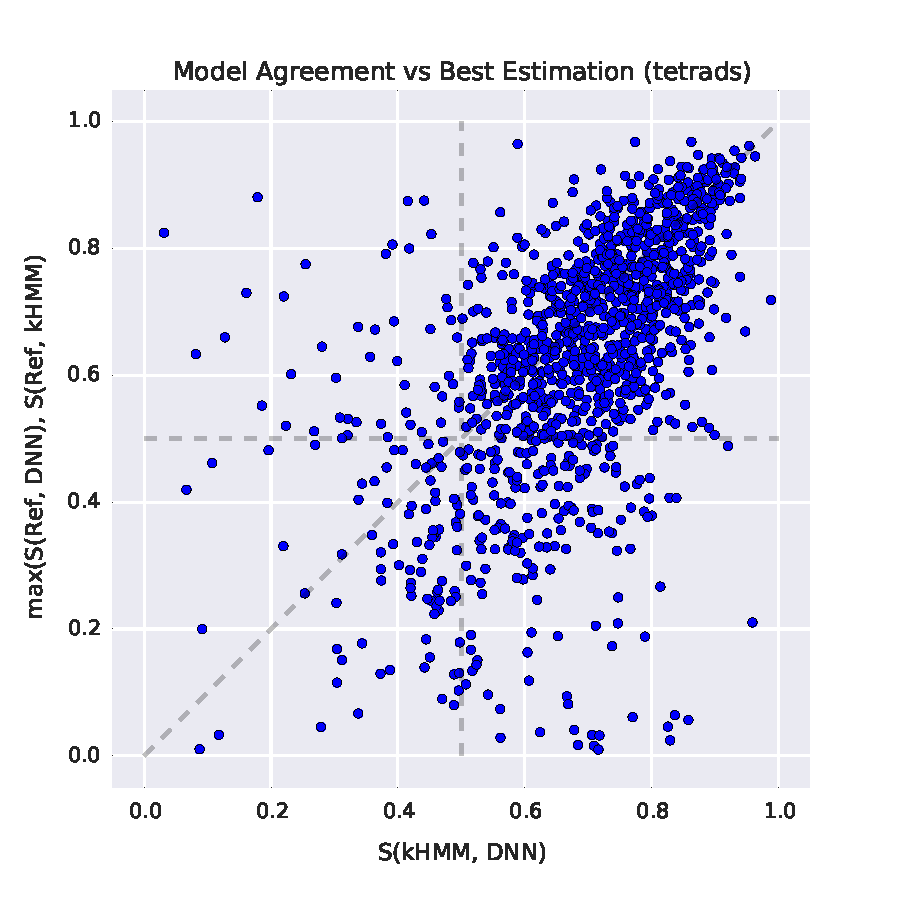
\includegraphics[width=0.9\columnwidth]{model_agreement-vs-best_est}
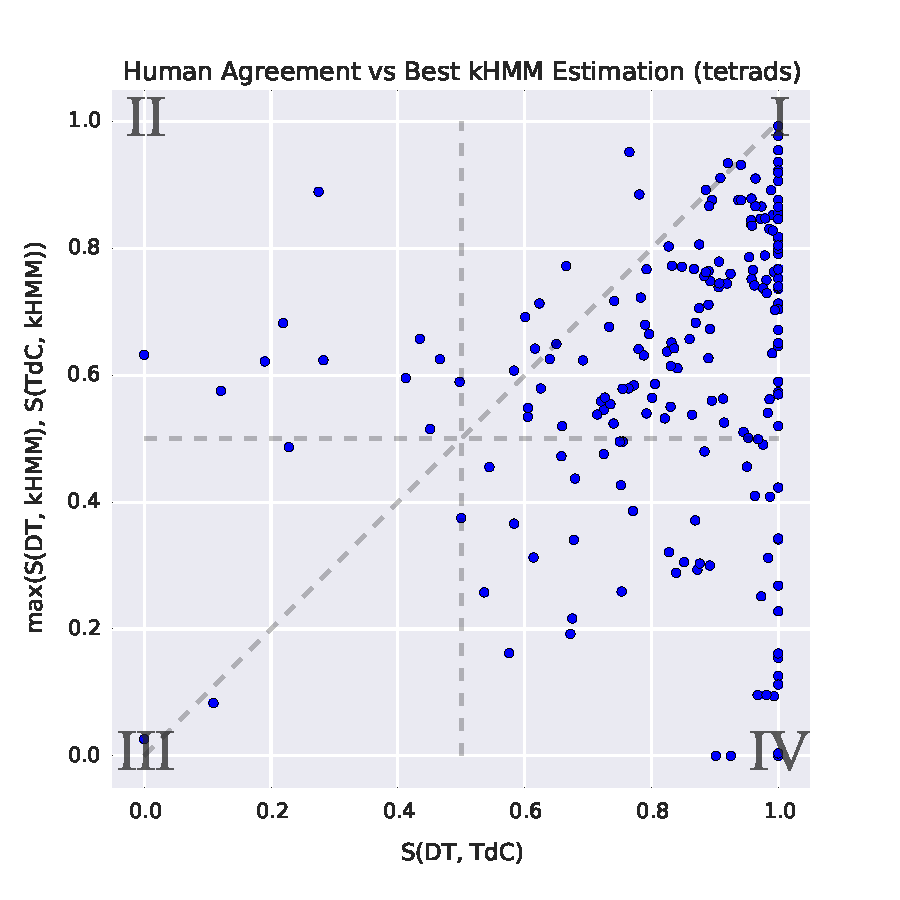
\includegraphics[width=0.9\columnwidth]{human_agreement-vs-best_kHMM_est}
\caption{Trackwise recall for the ``tetrads'' in two conditions: (top) over the ground truth data, illustrating \emph{model} agreement versus the better match between the reference and estimated annotations; (bottom) over the Rock Corpus data, illustrating annotator agreement versus the better match between the two reference and kHMM annotations.}
\label{fig:trackwise_recall}
\end{figure}

% Ground truth trackwise
Two track-wise scatter plots are given in \Cref{fig:trackwise_recall}, for the ground truth and Rock Corpus datasets.
The former compares the agreement between multiple \emph{estimations}, along $x$, with the better matching estimation for the given reference, along $y$, where each quadrant characterizes a different behavior:
(I), all annotations agree;
(II), one estimation matches the reference better than the other;
(III), all annotations disagree;
and (IV), the estimations agree more with each other than the reference.
Importantly, this track-wise comparison makes it easier to identify datapoints that can help address our original research questions.
Tracks for which only one algorithm performs well (II) likely indicate boundary chords.
Alternatively, instances where both algorithms produce poor estimations, and yet \emph{neither} agree (III), are curious and warrant further inspection.
Finally, tracks that result in similarly incorrect estimations (IV) highlight some kind of greater challenge to automatic systems.

The second plot, conversely, compares the agreement between multiple \emph{references}, along $x$, with the better matching reference for the given estimation, along $y$, and analogous characterizations by quadrant:
(I), all annotations agree;
(II), one reference matches the estimation better than the other;
(III), all annotations disagree;
and (IV), the references agree more with each other than the estimation.
Here, annotator disagreement in the presence of a matching estimation (II) is indicative of subjectivity, while disagreement between all annotations (III) is suspicious and should be explored.
Furthermore, tracks with an estimated annotation that fails to match either human perspective (III \& IV) likely identify room for improvement.


\section{Qualitative Analysis, in Four Parts}
\label{sec:analysis}

Using this suite of analysis tools described previously, a thorough exploration of the relationship between reference and estimated annotations is conducted, resulting in four significant insights.
In the spirit of both reproducibility and open access, a companion IPython notebook is made available online\footnote{\url{https://github.com/ejhumphrey/ace-lessons/experiments.ipynb}}, providing additional visualizations complementary to the following discussion.

\begin{figure*}[t!]
\centering
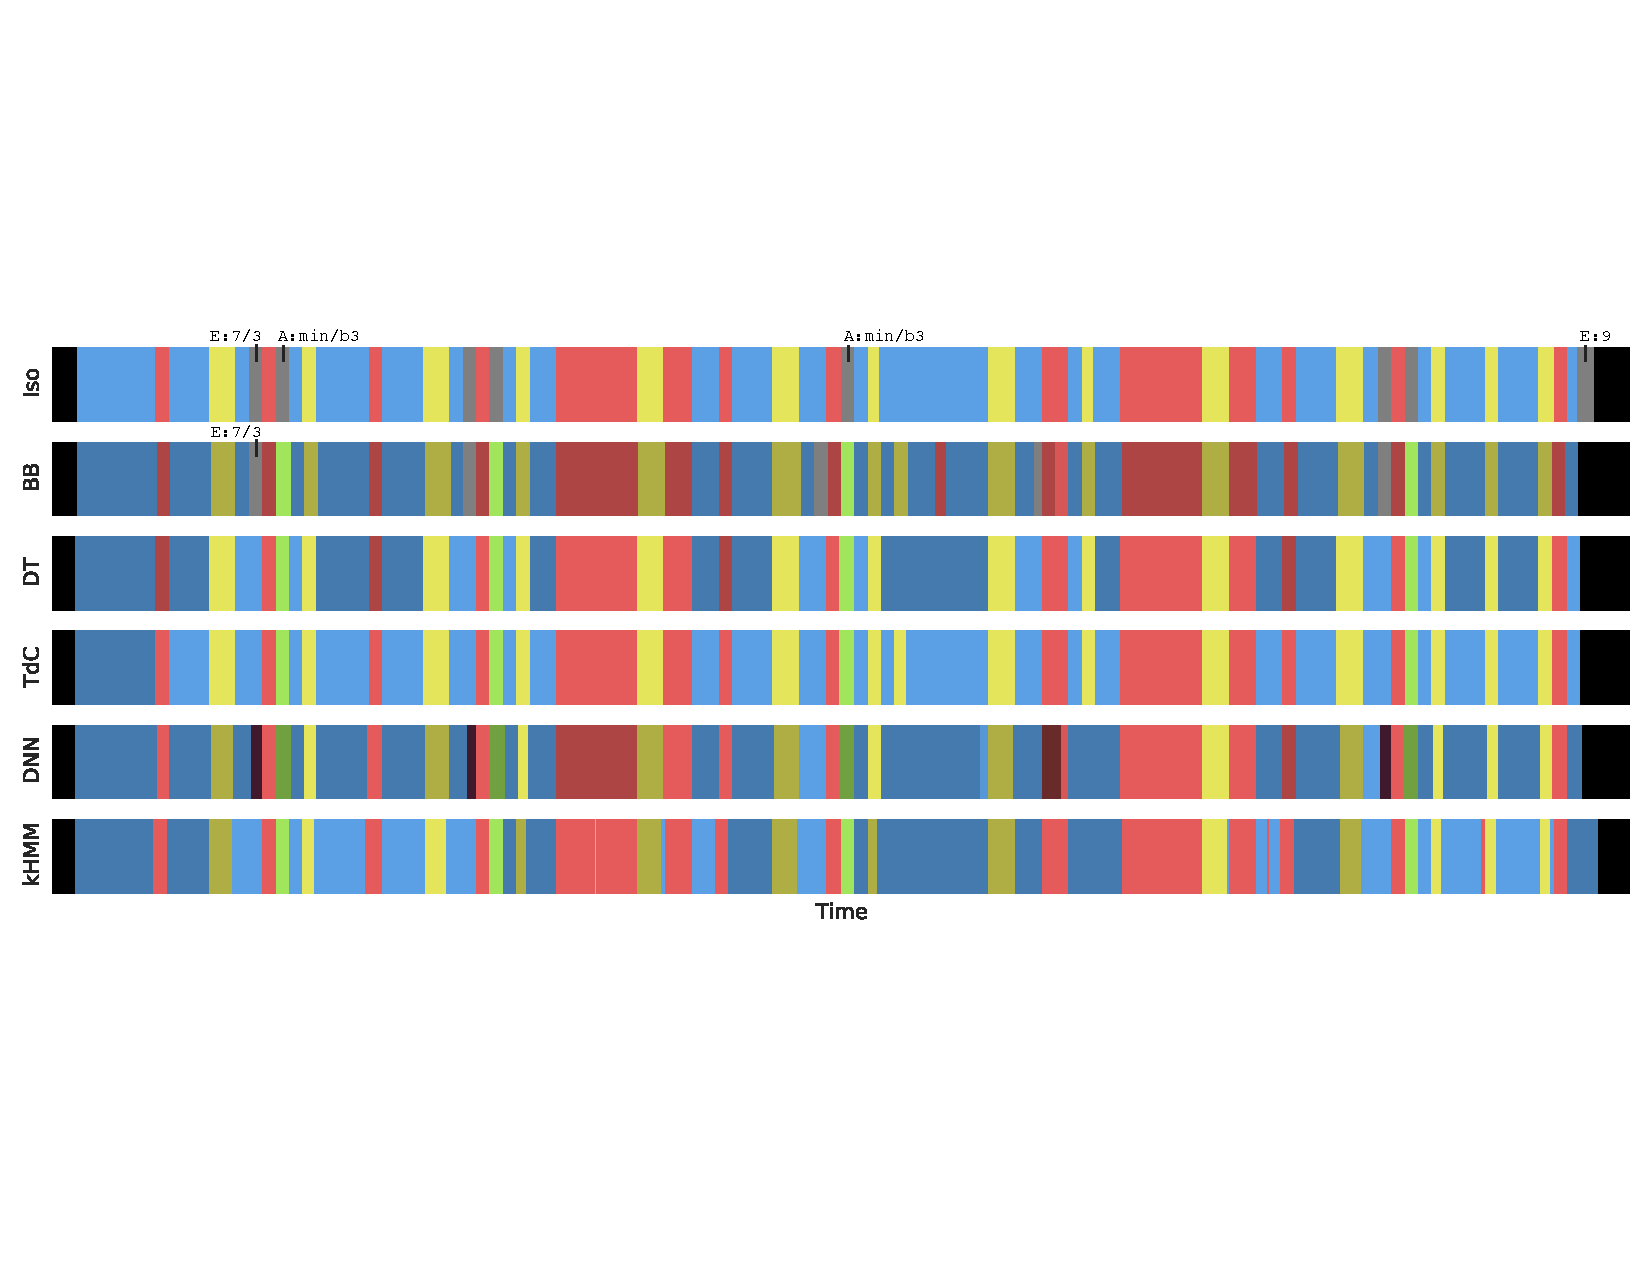
\includegraphics[width=\textwidth]{TROSSUK149E3AE03BD_annotations_mkup2}
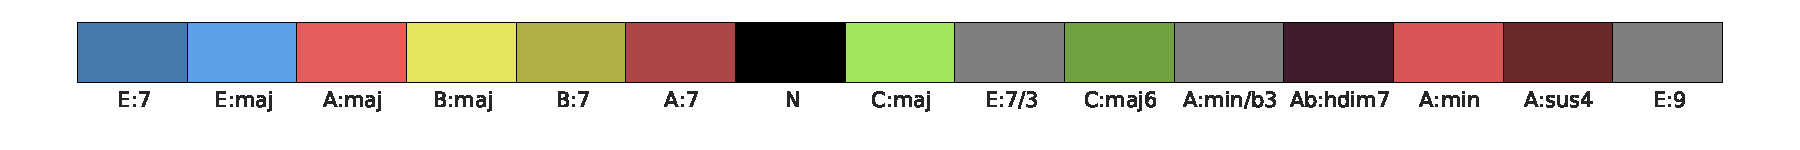
\includegraphics[width=\textwidth]{TROSSUK149E3AE03BD_legend}
\caption{Six perspectives on ``I Saw Her Standing There'', by \emph{The Beatles}, according to Isophonics (Iso), Billboard (BB), David Temperley (DT), Trevor deClercq (TdC), the Deep Neural Network (DNN), and the k-stream HMM (kHMM).}
\label{fig:beatles}
\end{figure*}


% Content Validity
\subsection{Invalid Harmonic Assumptions}
\label{subsec:validity}

An exploration of quadrant (IV) from \Cref{fig:trackwise_recall} reveals that a large source of error stems from musical content or reference chord annotations that violate basic assumptions about how chords are used.
One common form of this behavior is due to issues of intonation, where a handful of recordings are not tuned to A440, with some varying by more than a quarter-tone:
for example, ``Stand By Me'' by Jimmy Ruffin, ``I'll Tumble 4 Ya'' by \emph{The Culture Club}, ``Every Breath You Take'' by \emph{The Police}, or ``Nowhere to Run'' by Martha Reeves and \emph{the Vandellas}.
Understandably, as a result, the estimated annotations differ by a semitone from the reference, and perform poorly across all comparison rules.
% While the importance of tuning has been discussed previously in ACE research, this raises some interesting questions.
% Is it a meaningful obstacle to force automatic systems to compensate for imprecise tuning in an annotation, or a necessary assumption given the task of estimating absolute chord names?
% And furthermore, should evaluation measures be able to characterize ``good'' annotations that happen to be agnostic to key?

% Not all music is well described by chords.
The second observation finds that some tracks in the dataset do not truly make use of, and are thus not well described by, chords.
While a few classic songs by \emph{The Beatles} have been known to be of questionable relevance for their instrumentation and lack of standard chords, such as ``Revolution 9,'' ``Love You To,'' or ``Within You, Without You'', analysis here identifies several other tracks, spanning rap, hip hop, reggae, funk and disco, that behave similarly:
for example, ``Brass Monkey'' by \emph{The Beastie Boys}, ``I, Me, \& Myself'' by \emph{de la Soul}, ``Don't Push'' by \emph{Sublime}, ``Get Up (I Feel Like Being a Sex Machine)'' by James Brown, or ``I Wanna Take You Higher'' by Tina and Ike Turner.
This realization encourages the conclusion that chords may not be a valid way to describe all kinds of music, and that using such songs for evaluation may lead to erroneous or misleading results.

% A third and final relevant behavior is that many annotations consist of one and two note chords, e.g. \texttt{D:1/1}, \texttt{G:5}, or \texttt{A:maj(*3)}.


\subsection{Limitations of Chord Comparisons}

% Common manifestations in the data
The second observation resulting from this analysis is the difficulty faced in the comparison of related chords.
By and large, ACE systems are often forced to either map chords to a finite dictionary, or develop embedding rules for equivalence testing \cite{Raffel2014Eval}.
In either case, this quantization process assigns all observations to a one-of-$K$ representation effectively making all errors equivalent.
For the purposes of stable evaluation, this can have significantly negative consequences.

Chords are naturally related to each other hierarchically, and cannot always be treated as distinct classes.
Flat classification problems ---i.e. those in which different classes are disjoint--- are built on the assumption of mutually exclusive relationships.
In other words, assignment to one class precludes the valid assignment to any other class considered.
% For example, ``cat'' and ``dog'' are mutually exclusive classes of ``animal'', but ``cat'' and ``mammal'' are not.
In the space of chords, \texttt{C:dim7} and \texttt{C:maj} are perhaps mutually exclusive classes, but it is difficult to say the same of \texttt{C:maj7} and \texttt{C:maj}, as the former \emph{contains} the latter.
This conflict is a common source of disagreement between annotators of the Rock Corpus tracks, which are easily identified in or near the quadrant (II) of Figure \ref{fig:trackwise_recall}-b:
for example, ``Dancing In The Street'' by Martha Reeves \& The Vandellas, ``All Apologies'' by \emph{Nirvana}, or ``Papa's Got a Brand New Bag'' by James Brown.
In each case, the human perspectives each report related tetrads and triads, e.g. \texttt{E:7} and \texttt{E:maj}, causing low annotator agreement, while the machine estimation alternates between the two trying to represent both.
These kinds of errors are not ``confusions'' in the classic sense, but a limitation of evaluation methods to reliably quantify this behavior, and of the model to represent this naturally structured output.


% Alternatively, the flexibility of the standard chord syntax can be abused for ambiguous chords, and it isn't clear what to do with these labels.
% Occurrence of bizarre chord spellings in the data:
% Atypical chords often appear when the harmonic content isn't well described by chords.
% de la soul, etc.
% Hash pipe,
% Should these annotations exist?
% Unlikely that they will be used similarly by all annotators.


\subsection{Conflicting Problem Definitions}

Over the years, the automatic prediction of chord sequences from music audio has taken several names: estimation, recognition, identification, or transcription.
The analysis here motivates the notion that this is not merely a matter of semantics, but actually a subtle distinction indicative of two slightly different problems being addressed.
Chord \emph{transcription} is an abstract task related to functional analysis, taking into consideration high-level concepts such as long term musical structure, repetition, segmentation or key.
Chord \emph{recognition}, on the other hand, is quite literal, and is closely related to polyphonic pitch detection.
Both interpretations are easily found in the collection of reference annotations, however, conflating these two tasks to some unknown degree.

% A common manifestation of this challenge is found where silence, fades, or breaks in the song have been annotated as an actual chord.
% From the perspective of recognition, silence should always be labeled as ``no-chord.''
Furthermore, the goal in transcription is to assign chord labels to regions, and is closer in principle to segmentation than classic approaches to chord estimation.
One illustrative instance, ``All Apologies'' by \emph{Nirvana}, is identified in quadrant (II) of \Cref{fig:trackwise_recall}.
Here, the human annotators have disagreed on the harmonic spelling of the entire verse, with DT and TdC reporting \texttt{C\#:maj} and \texttt{C\#:7}, respectively.
On closer inspection, it would appear that both annotators are in some sense correct;
the majority of the verse is arguably \texttt{C\#:maj}, but a cello sustains the flat-$7^{th}$ of this key intermittently.
The regions in which this occurs are clearly captured in the estimated annotations, corresponding to its \texttt{C\#:7} predictions.
This proves to be an interesting discrepancy, because one annotator (DT) is using long-term structural information about the song to apply a single chord to the entire verse.


\begin{table*}[!t]
% increase table row spacing, adjust to taste
% \renewcommand{\arraystretch}{1.4}
% if using array.sty, it might be a good idea to tweak the value of
% \extrarowheight as needed to properly center the text within the cells
\small
\centering
\begin{tabular}{ c || c c c c | c c c c |}
Ver. & \multicolumn{4}{c}{Chord Sequence} & Score & Ratings & Views \\
 \hline
 Billboard & \texttt{D:maj} & \texttt{A:sus4(b7)} & \texttt{B:min7} & \texttt{G:maj9} & --- & --- & --- \\
 MARL & \texttt{D:maj} & \texttt{D:maj/5} & \texttt{D:maj6/6} & \texttt{D:maj(4)/4} & --- & --- & --- \\
 DT & \texttt{D:maj} & \texttt{A:maj} & \texttt{B:min} & \texttt{G:maj} & --- & --- & --- \\
 TdC & \texttt{D:maj} & \texttt{A:maj} & \texttt{B:min} & \texttt{G:maj} & --- & --- & --- \\
% \hline
DNN & \texttt{D:maj} & \texttt{A:sus4} & \texttt{B:min7} & \texttt{G:maj7} & --- & --- & --- \\
kHMM & \texttt{D:maj} & \texttt{A:sus4} & \texttt{B:min} & \texttt{G:maj} & --- & --- & --- \\
% \hline
1 & \texttt{D:maj} & \texttt{A:maj} & \texttt{B:min} & \texttt{G:maj} & 4/5 & 193 & 1,985,878 \\
2 & \texttt{D:5} & \texttt{A:sus4} & \texttt{B:min7} & \texttt{G:maj} & 5/5 & 11 & 184,611 \\
$3^*$ & \texttt{D:maj} & \texttt{A:maj} & \texttt{B:min} & \texttt{G:maj} & 4/5 & 23 & 188,152 \\
$4^*$ & \texttt{D:maj} & \texttt{A:maj} & \texttt{B:min} & \texttt{G:maj7} & 4/5 & 14 & 84,825 \\
$5^*$ & \texttt{D:maj} & \texttt{A:maj} & \texttt{B:min} & \texttt{G:maj} & 5/5 & 248 & 338,222 \\
6 & \texttt{D:5} & \texttt{A:5} & \texttt{D:5/B} & \texttt{G:5} & 5/5 & 5 & 16,208 \\
\hline
\end{tabular}
\caption{Various interpretations of the verse from ``With or Without You'' by \emph{U2}, comparing the reference annotations and automatic estimations with six interpretations from a popular guitar tablature website; a raised asterisk indicates the transcription is given relative to a capo, and transposed to the actual key here.}
\label{tab:wowu_chords}
\end{table*}


\subsection{Ground Truth \emph{vs.} Subjectivity}

While the role that subjectivity can play in chord estimation is becoming better understood \cite{Ni2013Understanding}, it is not handled gracefully in current ACE methodology, and there are two examples worth analyzing here.
The first, ``I Saw Her Standing There'' by \emph{The Beatles}, is given in Figure \ref{fig:beatles}, where the pitch class of the chord's root is mapped to color hue, and the darkness is a function of chord quality, e.g., all \texttt{E:*} chords are a shade of blue.
No-chords are always black, and chords that do not fit into one of the 157 chord classes are shown in gray.
Perhaps the most striking observation is the degree of variance between all annotations.
Based on the tetrads comparison, no two reference annotations correspond to greater than a 65\% agreement, with the DNN and kHMM scoring 28\% and 52\% against the ground truth Isophonics reference, shown at the top.
Despite this low score, the DNN and kHMM estimations agree with at least one of the four human annotations 89.1\% and 92.3\% of the song, respectively.
The two exceptions occur during the out-of-gamut chords, \texttt{E:7/3} and \texttt{A:min/b3}, which the DNN calls \texttt{Ab:hdim7} and \texttt{C:maj6}, respectively.
While both estimated chords share three pitches with the Isophonics reference, the other human annotators mark the \texttt{A:min/b3} instead as a root position \texttt{C:maj}.
Given how subjective it might be for human experts to agree on possible inversions, typical evaluation strategies may place too much emphasis on the root of a chord.

A second example to consider in the larger discussion of subjectivity is the verse of ``With or Without You'' by \emph{U2}.
Musically, one finds reasonably ambiguous harmonic content, consisting of a vocal melody, a moving bass line, a guitar riff, and a string pad sustaining a high-pitched \texttt{D}.
Complementing the four expert perspectives provided here, an Internet search yields six additional user-generated chord transcriptions from the website Ultimate Guitar\footnote{\url{http://tabs.ultimate-guitar.com/u/u2/with_or_without_you_crd.htm}, accessed 19 April 2015.}.
All human perspectives and both machine interpretations are consolidated in Table \ref{tab:wowu_chords}, noting both the average and number of ratings, as well as the number of views the public chord annotation has received.
Though view count is not directly indicative of a transcription's accuracy, it does provide a weak signal indicating that users did \emph{not} rate it negatively.

This particular example provides several valuable insights.
Nearly all perspectives are equivalent at the major-minor level, with the exception of the MARL annotation, which differs only slightly.
That said, the differences between user-generated annotations do not noticeably impact the average ratings.
This is an important consideration when building user systems, whereby objective measures are valuable insofar as they correlate with subjective experience.
Similarly, these annotations are indicative of, at least for this song, a preference for root position chords.
Thus, subjectivity plays a role in the collection of reference annotations, as well as the end-user experience.


\section{Conclusions and Future Perspectives}
\label{sec:perspectives}

In this work, qualitative analysis of system performance led to the identification of four key observations affecting current chord estimation methodology:
one, not all music content is valid in the context of chord estimation;
two, conventional comparison methods struggle to accurately characterize the complex relationships between chords;
three, conventional methodology has mixed the somewhat conflicting goals of chord transcription and recognition to an undefined degree;
and four, the subjective nature of chord perception may render objective ground truth and evaluation untenable.

% For chord estimation
% * Subjectivity should be embraced
% * Tagging is an option
% * Parallels to segmentation
Looking to the future of automatic chord estimation, a few opportunities stand out.
First and foremost, subjectivity in reference annotations should be embraced rather than resolved.
Chord estimation may be better understood as a time-aligned ``tagging'' problem, modeled as multinomial regression, or as structured prediction.
Furthermore, synthesizing multiple human perspectives into a continuous-valued chord affinity vector would allow for more stable evaluation by encoding the degree to which a chord label applies to an observation.
From a system design perspective, chord transcription, as a disctinct task, stands to benefit greatly from recent advances in music structure analysis.
To the point, however, it is also crucial to distinguish between the different flavors of harmonic analysis, and how a collection of reference data does ---or does not--- reflect the specific problem being addressed.

% For content-based MIR
% * Can't blindly throw powerful models at a problem; sometimes domain knowledge to understand what the system is doing and why.
% * Subjective evaluation of MIR systems is necessary;
% ** Make sure you haven't drifted from the goal
% ** Don't lose sight of the things you're really trying to solve.
% * Bootstrap good systems to collect more reference data; correction is often easier than open-ended annotation
In a more general sense, this inquiry also has implications for the larger field of content-based MIR.
Perhaps most presssing, the most powerful model cannot compensate for methodological deficiencies, and domain knowledge can be crucial to help understand system behaviour.
Similarly, qualitative evaluation should play a larger role in the assessment of automatic systems intended for user-facing applications.
If nothing else, users studies can help identify objective measures that align well with subjective experience.
Finally, on a more practical note, high-performing systems can and should be used to facilitate the curation of reference annotations.
These systems can be used to solicit human perspectives at a much larger scale, for both new and previously annotated content.


\bibliography{library}


\end{document}
